\hypertarget{_s_c_p_i__regs_8h}{\section{scpi/\-S\-C\-P\-I\-\_\-regs.h File Reference}
\label{_s_c_p_i__regs_8h}\index{scpi/\-S\-C\-P\-I\-\_\-regs.\-h@{scpi/\-S\-C\-P\-I\-\_\-regs.\-h}}
}
This graph shows which files directly or indirectly include this file\-:\nopagebreak
\begin{figure}[H]
\begin{center}
\leavevmode
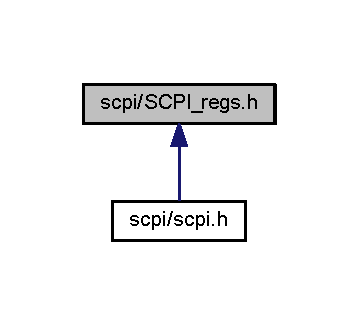
\includegraphics[width=172pt]{_s_c_p_i__regs_8h__dep__incl}
\end{center}
\end{figure}


\subsection{Detailed Description}
This file creates the S\-C\-P\-I required registers such as S\-T\-B and Questionable and provides the functions for managing them

Some bits of the status byte, questionable and operation registers are available to the application designer. See the I\-E\-E\-E Std 488.\-2 and S\-C\-P\-I-\/99 for details on the operation of these registers.

This file should not need to be edited by the user.

\begin{DoxySeeAlso}{See Also}
\hyperlink{_s_c_p_i__specific_regs_8h}{S\-C\-P\-I\-\_\-specific\-Regs.\-h} 
\end{DoxySeeAlso}
